Este capítulo presupone que en el ordenador está instalado Traverso \Version\ o posterior. Si no es así, por favor consulte el capítulo \ref{sect_installation} . 

Puede lanzar Traverso desde el menú principal, o pulsando Alt-F2 y tecleando \texttt{traverso} en el área de comandos. Lo primero que verá será una ventana de diálogo preguntándole por el directorio de proyectos. Si aún no hay ninguno, cree uno nuevo. Este directorio contendrá todos los proyectos, incluyendo los archivos de audio. Tenga en cuenta que si va a hacer trabajos serios de audio, necesitará \emph{mucho} espacio de disco. Entre en el directorio y pulse OK. Tras confirmar su selección, se mostrará la ventana principal de Traverso. Esta contiene diferentes regiones que son sensibles a la "selección blanda". En \FigT\ \ref{fig_gui01} se muestra la nomenclatura usada en este manual. 

\begin{figure}
 \centering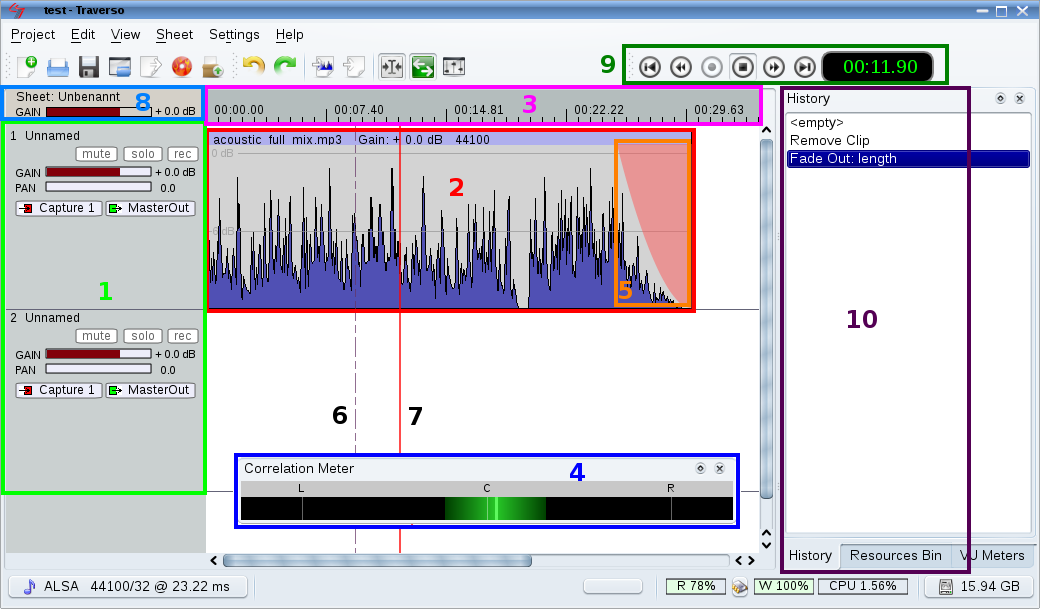
\includegraphics[width=\textwidth]{../images/sshot06.png}
 \caption{Elementos en la pantalla de Traverso. 1 Panel de pistas: Si el ratón se desplaza a este área, las acciones de teclado se aplicarán a la pista que esté bajo el ratón. 2 Clip de Audio: Las acciones de teclado se aplican al clip de audio. 3 Línea de Tiempo: Las acciones de teclado se aplican a los marcadores en la línea de tiempo. 4 Ventanas y Accesorios acoplables. 5 Fade de salida. 6 Cursor de trabajo. 7 Cursor de reproducción. 8 Area de la hoja. 9 Consola clásica de transporte. 10 Historia de comandos.}
 \label{fig_gui01}
\end{figure}

Las herramientas de Traverso usan ventanas acoplables, lo que permite elegir su disposición como se desee. Simplemente pulse en la barra de título para arrastrar la ventana elegida a una posición nueva. Es posible apilar los accesorios unos sobre otros, o separarlos de la ventana principal para moverlos libremente. Esto último es particularmente útil cuando se usan dos monitores: la ventana principal puede ocupar un monitor, y los accesorios estar en el otro (\FigB\ \ref{fig_mainwin02}).

\begin{figure}
 \centering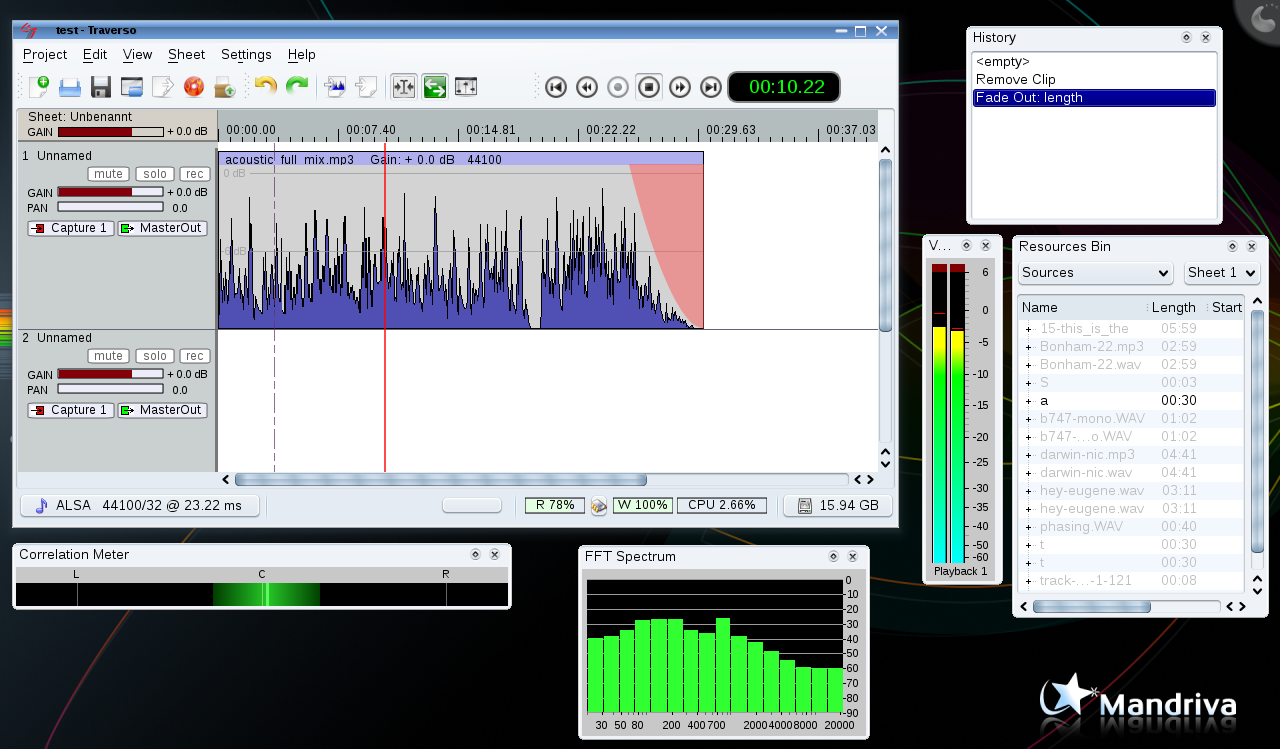
\includegraphics[width=\textwidth]{../images/sshot03.png}
 \caption{Las ventanas acoplables pueden separarse de la ventana principal. Y pueden moverse a otro monitor, si se dispone de varios.}
 \label{fig_mainwin02}
\end{figure}

\section{Soporte de Drivers}
Traverso puede funcionar sobre cuatro drivers distintos: el driver Null, el driver ALSA, el servidor de sonido Jack, y el driver PortAudio (en Windows y Mac OS X). Seguidamente se explica cuáles son las ventajas y desventajas de cada uno, y cómo configurarlos correctamente. En la barra de información del sistema se muestra el driver que está cargado en cada momento.

\subsection{Driver Null}

\includegraphics[height=\baselineskip]{../images/tux.png}

\includegraphics[height=\baselineskip]{../images/mac.png}

\includegraphics[height=\baselineskip]{../images/win.png}
\\
El driver Null se carga automáticamente cuando ningún otro driver está disponible, pero no se puede escuchar nada mientras se esté utilizando este driver. Por tanto, seguramente no querrá nunca cargar este driver manualmente. Para seleccionar un driver válido, pulse sobre la etiqueta \emph{Null Driver} para abrir una ventana de configuración \FigB\ \ref{fig_driverconf}).

\subsection{ALSA}

\includegraphics[height=\baselineskip]{../images/tux.png}
\\

Al seleccionar ALSA, Traverso se comunica directamente con el servidor de sonido ALSA, lo que sólo es posible si ninguna otra aplicación lo está usando. Por tanto, debe detener la reproducción de sonido de cualquier otra aplicación antes de seleccionar este driver. Compruebe también que la bandeja del sistema (Gnome/KDE) no esté ejecutando en modo minimizado Amarok, XMMS, etc. En la pantalla de configuración del driver de Traverso, elija el driver \emph{ALSA}, la frecuencia de 44100, y deje el valor por defecto de la latencia. Presione \emph{OK} y compruebe que la etiqueta del driver ha cambiado a \emph{ALSA}. Si el nuevo driver no se carga, la tarjeta de sonido puede estar aún ocupada por otra aplicación. Vuelva a comprobar que se detuvieron todas las aplicaciones multimedia, y que el daemon de audio (por ej. aRTs) se apaga automáticamente cuando no está en uso. Después vuelva a intentar cargar el driver ALSA. Si es aceptado como driver válido, es que se ha configurado correctamente.

\subsection{Jack}

\includegraphics[height=\baselineskip]{../images/tux.png}

\includegraphics[height=\baselineskip]{../images/mac.png}
\\

Traverso puede conectarse también al servidor de sonido Jack, que proporciona funciones de enrutación avanzadas, y conexión con latencia cero entre clientes (si usted no necesita estas funciones, y ALSA le funciona bien, no hay necesidad de usar Jack). Recomendamos usar \emph{qjackctl}, que permite configurar Jack fácilmente. Lance el daemon de jack pulsando \emph{Start} en qjackctl. Cuando esté corriendo, conecte el driver \emph{jack} desde la ventana de configuración de Traverso (\FigB\ \ref{fig_driverconf}), y pulse \emph{OK}. La barra debiera mostrar la etiqueta \emph{jack} si el driver se carga correctamente. Ahora vuelva a qjackctl y abra la ventana \emph{Conectar}. \emph{Importante:} Debe realizar la conexión manualmente para poder escuchar sonido. Seleccione Traverso en la parte izquierda (``Clientes Leíbles''), y alsa\_pcm en la parte derecha (``Clientes escribibles''). Después pulse \emph{conectar}. Si todo va bien, se dibujará una línea conectando ambos clientes.


\begin{figure}
 \centering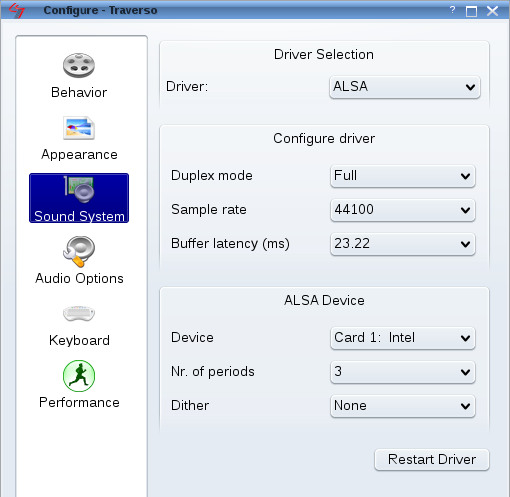
\includegraphics[width=0.5\textwidth]{../images/sshot02.png}
 \caption{El driver de audio puede seleccionarse desde el menú. Traverso funciona con ALSA, Jack, Portaudio, y tiene un driver {Null} como solución de emergencia, para momentos en que no haya otro driver que funcione.}
 \label{fig_driverconf}
\end{figure}

\subsection{Port Audio}

\includegraphics[height=\baselineskip]{../images/mac.png}

\includegraphics[height=\baselineskip]{../images/win.png}
\\

Port Audio es el driver recomendado para Mac OS X y Microsoft Windows. Se conecta al sistema de audio nativo (CoreAudio en OS X, WMME en Windows). Simplemente seleccione ``PortAudio'' en la ventana de configuración del driver, la frecuencia de muestreo que quiera usar, y un valor de la latencia adecuado a la capacidad de su ordenador.

\section{Formato de Archivo para Grabación}
En el menú ``Ajustes $\rightarrow$ Formato de Archivo para Grabación'' puede especificar el formato de archivo en el que almacenará el audio. \emph{Wave} viene siendo el formato estándar. El audio no se comprime, y Traverso lo guarda en coma flotante de 32 bits, sin importar la profundidad de bits elegida en el driver. Sin embargo, estos archivos están limitados a un tamaño de unos 4 Gb. Para una grabación mono de 44100 Hz, 32 bit, esto implica un tiempo máximo de grabación de 6h 45 min. En una grabación stereo, el límite es la mitad, unas 3h 23 min. Aunque esto es suficiente en muchos casos, puede ser una limitación al grabar a tasas de muestreo mayores. En el caso de grabación stereo a 192 kHz, 32 bit, la limitación de tiempo es 45 min. La limitación de 4 Gb puede evitarse usando el formato \emph{Wave-64}, que es un formato de 64 bits reales capaz de guardar archivos mucho mayores que 4 Gb. El tercer formato, \emph{WavPack}, usa un algoritmo de compresión sin pérdidas para reducir el tamaño de los archivos sin afectar a la calidad del audio. Sin embargo, como la codificación se hace en tiempo real, se requiere más uso de CPU durante la grabación. Si le preocupa el espacio en disco pero tiene una CPU rápida, este formato es una buena elección.

